% Filename: sets03@tikz_for_teachers.tex
% This code is part of LaTeX with Vim.
% 
% Description: TikZ for teachers is free book about TikZ and Sage.
% 
% Created: 30.03.12 08:12:04 PM
% Last Change: 30.03.12 08:12:56 PM
% 
% Author: Raniere Gaia Costa da Silva, r.gaia.cs@gmail.com
% Organization:  
% 
% Copyright (c) 2010, 2011, 2012, Raniere Gaia Costa da Silva. All rights 
% reserved.
% 
% This file is license under the terms of a Creative Commons Attribution 
% 3.0 Unported License, or (at your option) any later version. More details
% at <http://creativecommons.org/licenses/by/3.0/>.
% Set operations illustrated with Venn diagrams
% Author: Uwe Ziegenhagen
% This is an expanded version of an example provided by T. Tantau

% Definition of circles
\def\firstcircle{(0,0) circle (1.5cm)}
\def\secondcircle{(0:2cm) circle (1.5cm)}

\colorlet{circle edge}{blue!50}
\colorlet{circle area}{blue!20}

\tikzset{filled/.style={fill=circle area, draw=circle edge, thick},outline/.style={draw=circle edge, thick}}

\setlength{\parskip}{5mm}
% Set A and B
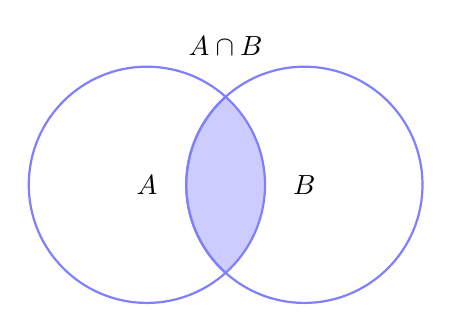
\begin{tikzpicture}
    \begin{scope}
        \clip \firstcircle;
        \fill[filled] \secondcircle;
    \end{scope}
    \draw[outline] \firstcircle node {$A$};
    \draw[outline] \secondcircle node {$B$};
    \node[anchor=south] at (current bounding box.north) {$A \cap B$};
\end{tikzpicture}

%Set A or B but not (A and B) also known a A xor B
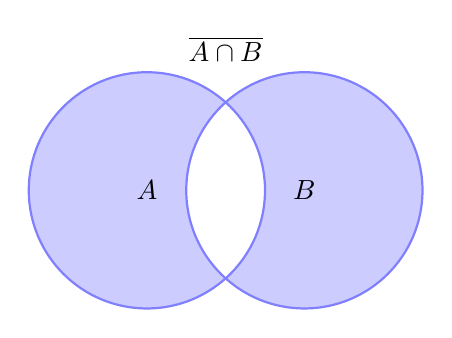
\begin{tikzpicture}
    \draw[filled, even odd rule] \firstcircle node {$A$}
    \secondcircle node{$B$};
    \node[anchor=south] at (current bounding box.north) {$\overline{A \cap B}$};
\end{tikzpicture}

% Set A but not B
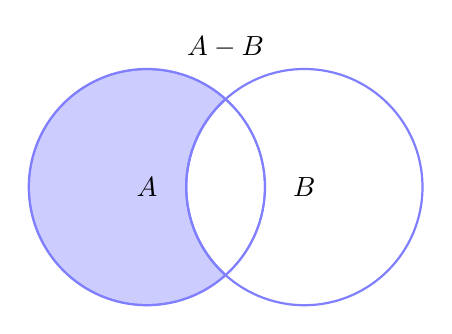
\begin{tikzpicture}
    \begin{scope}
        \clip \firstcircle;
        \draw[filled, even odd rule] \firstcircle node {$A$}
        \secondcircle;
    \end{scope}
    \draw[outline] \firstcircle
    \secondcircle node {$B$};
    \node[anchor=south] at (current bounding box.north) {$A - B$};
\end{tikzpicture}
